\documentclass[12pt]{article}

\usepackage{sbc-template}
\usepackage{indentfirst}
\usepackage{graphicx,url}
\usepackage{float}
\usepackage{url}
\usepackage[brazil]{babel}   
%\usepackage[latin1]{inputenc}  
\usepackage[utf8]{inputenc}  
% UTF-8 encoding is recommended by ShareLaTex

     
\sloppy

\title{\textit{Naïve Bayes} e \textit{Support Vector Machines}: Uma Análise Comparativa}

\author{Gustavo Zanoni Felipe\inst{1}, Mariana Soder\inst{1}}


\address{Universidade Estadual de Maringá (UEM) -- Maringá (PR)
  \email{ra\{92821,95381\}@uem.com.br}
}

\begin{document} 

\maketitle
     
\begin{resumo} 
    Em um cenário de classificação, muitos algoritmos classificatórios podem ser escolhidos de acordo com o problema. Dentre as possibilidades, está o algoritmo de \textit{Naïve Bayes}. Este, deriva-se do teorema de probabilidade de \textit{Bayes} para prever uma classe de um conjunto de dados desconhecidos. Uma outra alternativa seria utilizar de \textit{Support Vector Machines} (SVM). Um algoritmo, que tenta dividir padrões de amostras de uma base de dados por meio de um hiperplano. Em uma situação hipotética, onde trabalha-se em um problema de classificação, tendo as variáveis do problema analisadas e um curto período de tempo para obter resultados, uma solução eficiente seria a de utilizar classificadores derivados da regra de \textit{Bayes}. Estes, apresentam-se como eficientes e muitas vezes mais rápidos que demais classificadores. O algoritmo SVM por outro lado, nos últimos tempos vem obtendo um grande destaque devido ao seu bom desempenho em tarefas de classificação nos mais diversos domínios da aplicação. Tendo isto em mente, este trabalho visou realizar uma análise comparativa entre uma nova implementação do algoritmo classificatório \textit{Naïve Bayes} e uma versão da literatura do algoritmo \textit{Support Vector Machines} (SVM). Para que isso fosse realizado, três bases de dados foram utilizadas. Estas, foram divididas em 10 \textit{folds} (de acordo com a técnica do \textit{k-folds cross-validation}) e classificados com ambos algoritmos. Os resultados foram anotados e a partir deles, foram montadas as matrizes de confusão. Estas foram utilizadas para que a análise das classificações fossem avaliadas. Ao fim deste trabalho, o algoritmo de classificação aqui desenvolvido de \textit{Naïve Bayes} obteve um melhor desempenho que o algoritmo SVM. Dentre as métricas de avaliação empregadas, este obteve valores relativamente melhores, onde no melhor dos casos a diferença de acurácia para uma determinada base foi de 6,04\%. Das base de dados utilizadas, a que obteve um melhor desempenho alcançou 100\% de acurácia. Tal valor pode ser justificado pela disposição da base, onde a mesma possui apenas duas classes, as quais possuem diferenças discrepantes em suas amostras e estas possuem um baixo nível de variabilidade.
\end{resumo}


\section{Introdução}
    Imagine o seguinte cenário, você é estudante de ciência da computação e em um dos trabalhos do curso, você deve realizar uma tarefa de classificação. Você já coletou os dados da base e os analisou, averiguando a correlação entre seus atributos e a frequência que eles aparecem. Porém, como todo bom estudante você começou a realizar este trabalho um dia antes de sua data limite de entrega. Com a quantidade de amostras na base de dados, você precisa de um método rápido de classificação para que seja possível conseguir resultados em pouco tempo. Uma boa alternativa, seria utilizar o algoritmo de classificação \textit{Support Vector Machines}, devido ao seu sucesso em inúmeras tarefas de classificação presentes na literatura. Uma outra alternativa para o problema recém descrito seria o de utilizar um classificador derivado da Regra de Bayes, já que esse, mostra-se eficiente e rápido.
    
    A Regra de Bayes é uma equação simples e muito utilizada em sistemas inteligentes modernos. A partir dela é possível criar algoritmos classificadores e Redes inteiras, com a possibilidade de exprimir relações condicionais e de independência entre as variáveis do problema abordado. Um classificador conhecido que usufrui da Regra de Bayes, é o Naïve Bayes. Este trata cada atributo de uma amostra como sendo independente dos demais. Com base na frequência dos valores dos atributos em relação às classes apresentadas, é possível realizar predições de forma eficiente e rápida. De outra forma, o algoritmo de Classificação \textit{Support Vector Machines} divide os padrões de amostras presentes em uma base de dados por meio de uma reta chamada de hiperplano. Em problemas onde os padrões possuem difícil divisão em seu espaço dimensional original, é possível utilizar do \textit{Kernel Trick}, onde uma dimensão é adicionada ao problema. Assim, facilitando a divisão de tais padrões.
    
    Tendo isto em base, este trabalho visou realizar uma análise comparativa entre dois algoritmos classificadores. Sendo estes uma versão aqui implementada de Naïve Bayes e o algoritmo \textit{Support Vector Machines} da biblioteca \textit{sci-kit learn}. Para que isto fosse realizado, três bases de dados retiradas do repositório \cite{Dua:2017} foram utilizadas em um esquema de classificação, o qual realizava \textit{cross-validation} utilizando-se 10 \textit{folds}. Ao final, os resultados foram analisados tendo em base as matrizes de confusão geradas.
    
    O resto deste trabalho está organizado como descrito: a Seção \ref{classi} apresenta o conceito de classificação e os agoritmos de classificação utilizados. A Seção \ref{expandaval} apresenta os conceitos relacionados às métricas de avaliação de classificadores. A Seção \ref{mat} apresenta os materiais e métodos utilizados neste trabalho. A Seção \ref{resul} apresenta os resultados encontrados neste trabalho, enquanto a Seção \ref{conclu} conclui este trabalho.
    
\section{Classificação} \label{classi}
    Dentro do contexto da inteligência artificial, podem ser definidos diversos tipos de aprendizados. Como por exemplo, aprendizado supervisionado, não-supervisionado, semi-supervisionado e etc. No aprendizado supervisionado, o agente observa alguns exemplos de pares de entrada/saída e aprende a função que mapeia a entrada à saída. Neste caso, o valor da saída é disponível diretamente do preceitos do agente. 
    
    Logo a tarefa do aprendizado supervisionado se baseia em dado um conjunto de treino de \textit{n} exemplos de pares de entrada/saída $(x_1, y_1), (x_2, y_2), ..., (x_n, y_n),$, descobrir uma hipótese (função $h$)  que se aproxima de uma função verdadeira $f$ que gera cada um dos valores $y_i$, i. e. $y = f(x)$. Para avaliar o desempenho da hipótese, é dado um conjunto de teste de exemplos distintos daqueles utilizados no conjunto de treino.
    
    Problemas de aprendizado supervisionado podem ser divididos em de classificação ou regressão, onde estes diferenciam-se pelo tipo de saída. Caso as possibilidades de uma saída $y$ estejam presentes em um conjunto finito de valores, o problema é categorizado como classificação (booleana/binária caso este conjunto seja de dois valores). De outro modo, se $y$ assume um valor numérico, este categoriza-se como um problema de regressão \cite{norvig}.

    Um classificador pode ser assumido como uma função que designa a \textit{label} de uma classe $C$ existente em \{$C_1, ..., C_m$\} à um objeto descrito por um conjunto de atributos $X = {X_1, ..., X_n}$ . Desta forma, classificadores estatísticos tratam os atributos X e as classes C como variáveis randômicas, que são definidas pela sua função de densidade probabilística \cite{bnc}.

    \subsection{Naive-Bayes} \label{class}
        % Definir a regra de Bayes e explicar seu uso
        Segundo \cite{norvig} a regra de \textit{bayes} foi assim denominada em homenagem a Thomas Bayes (11702-1761) que introduziu a regra de raciocínio sobre probabilidades condicionais.
        
        Ainda segundo o autor, a regra é uma equação simples, porém, base de todos os sistemas modernos de inteligência artificial para inferência probabilística. Sendo ela apresentada na equação \ref{eq1}.
                
        \begin{equation} \label{eq1}
            P(X | Y) = \frac{P(Y | X) * P(X)}{P(Y)}
        \end{equation}
                
        Através da equação, pode-se perceber que ela nos permite calcular o termo $P(X | Y)$ em termos de três termos: $P(Y | X)$, P(X) e P(Y). A princípio tal regra não parece tão útil, porém, estes três termos geralmente são encontrados de uma maneira fácil e o que estima-se calcular é o quarto número. Sendo assim, podemos dizer que a regra de \textit{bayes} permite que probabilidades desconhecidas sejam calculadas a partir de probabilidades condicionais conhecidas.
    
        Neste contexto, classificadores Bayesianos identificam um objeto de acordo com a maior probabilidade posterior. Logo, a classe de um objeto é determinada pelo teorema de Bayes. Segundo este mesmo raciocínio, descreve-se o Classificador de Naïve Bayes. Este, determina que todos os atributos são condicionalmente independentes de uma determinada classe. 
        
        A regra de classificação de Naïve-Bayes, observada pela equação \ref{nbclass}, descreve que uma classe de um objeto pode ser predita pela probabilidade máxima encontrada entre as predições calculadas variando-se as classes ao realizar-se uma multiplicação da probabilidade de ocorrências de uma classe C com o produtório da regra de Bayes dos atributos para esta mesma classe.
    
        \begin{equation}\label{nbclass}
            pred = \arg\max P(c_j)\prod^{n}_{i=1}P(X_i = x_i | c_j)
        \end{equation}
        
        Para que tal regra seja calculada, é necessário encontrar a probabilidade de uma determinada classe C. Para que isso ocorra, precisa-se realizar o cálculo apresentado na equação \ref{pc}. Este valor é alcançado pela divisão do número de amostras pertencentes à uma determinada classe C pelo número total de amostras presentes em uma base de dados.
        
        \begin{equation}\label{pc}
           P(c_j) = \frac{N_j}{N}
        \end{equation}
        
        Para estimar o valor da regra de Bayes para este contexto, utiliza-se a equação \ref{pxc}. Esta, pode ser interpretada como a divisão do número de exemplos de uma classe $C_j$ que possuem um valor $x_k$ em seu atributo $X_i$ pela quantidade de amostras desta mesma classe $C_j$ \cite{bnc}.
        
        \begin{equation}\label{pxc}
           P(X_i = x_k | c_j) = \frac{N_{ijk}}{N_j}
        \end{equation}
        
    \subsection{Support Vector Machines}
    
    Segundo \cite{bohra}, \textit{Support Vector Machines} (SVM) são algoritmos de aprendizagem supervisionada que podem ser usados para classificar dados tanto com classes binárias quanto com classificações que contenham multiclasses. 
    
    A ideia principal é procurar uma função que separe os dados em suas categorias e que os mesmos possam ser desenhados como hiperplanos.
    Para minimizar o erro de teste e para melhorar a precisão da classificação, o SVM utiliza a função \textit{kernel}, que transforma os dados em um espaço de alta dimensão, onde os dados podem ser separados linearmente e para poder classificá-los de acordo com seus atributos \cite{bohra}.
    
    Segundo a documentação do \textit{scikit-learn}\footnote{https://scikit-learn.org/stable/\_downloads/scikit-learn-docs.pdf}, as classes SVC, nuSVC e LinearSVC são capazes de executar classificações de um conjunto de dados com multiclasses.
    
    A figura \ref{fig:svm} mostra exemplos de alguns classificadores citados. Nela, pode-se observar exemplos de classificação com as classes SVC e LinearSVC com diferentes tipos de \textit{kernel}. 
    
    \begin{figure}[h]
        \centering
        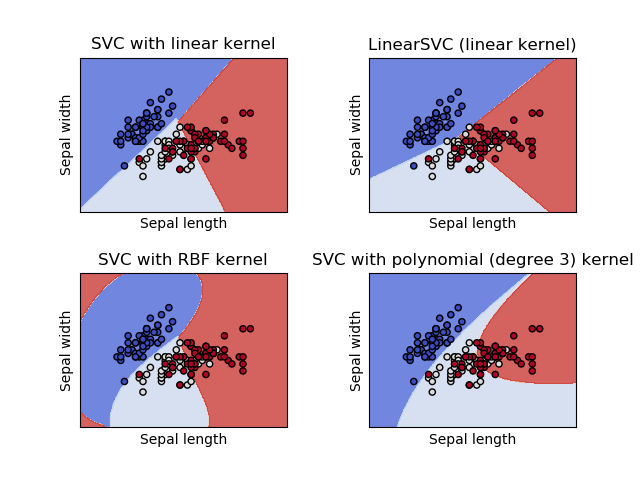
\includegraphics[width=.85\textwidth]{svc.png}
        \caption{Exemplo de classificadores SVM da classe SVC e LinearSVC utilizando diferentes \textit{kernels} implementados pela biblioteca \textit{scikit-learn} Imagem retirada de \cite{scikit-learn}.}
        \label{fig:svm}
    \end{figure}
    
    Para este trabalho, a escolha foi de utilizar o classificador LinearSVC da biblioteca \textit{scikit-learn}. 

\section{Métricas de Avaliação} \label{expandaval}
    Para a separação das bases em teste e treino, foi utilizada a técnica \textit{k-fold cross-validation}, que divide o conjunto de dados $D$ aleatoriamente, em $k$ subconjuntos (\textit{folds}) $D1, D2,..., Dk$ de tamanho aproximadamente igual. O indutor é treinado e testado $k$ vezes; onde em cada tempo $t \in \{1,2,...,k\}$, o indutor é treinado com o conjunto $D$ excluíndo-se o $Dt$ e testado com $Dt$ \cite{kohavi}.
    
    Ainda segundo \cite{kohavi} um bom número pra o valor de \textit{k} seria dez. Sendo este o escolhido para a realização de experimentos neste trabalho.
    
    Desta forma, tendo as predições calculadas por meio das classificações, é possível montar a matriz de confusão. Esta, baseia-se em uma matriz \textit{N}*\textit{N} (onde \textit{N} é o número de classes presentes no problema abordado) que possibilita observar a quantidade de predições realizadas para cada classe em relação às outras. 
    
    A partir desta, é possível calcular diferentes valores de probabilidade que avaliam a classificação realizada. Dentre as aqui utilizadas, estão:
        
    \begin{itemize}
        \item Acurácia: define no geral, o quão frequente o classificador está correto;
        \item Precisão: dentre as predições corretas, quantas efetivamente eram de tal natureza;
        \item \textit{Recall}: calcula a frequência em que o classificador encontra os exemplos de uma determinada classe;
        \item F1-Score: indica a qualidade geral do sistema de classificação desenvolvido, utilizando da combinação da precisão e \textit{recall}.
    \end{itemize}

\section{Materiais e Métodos}\label{mat}
Nesta seção apresentaremos os materiais, como as bases de dados utilizada para o trabalho, assim como algumas métricas de avaliação aplicadas ao final dos experimentos.

    \subsection{Bases de Dados}
        As bases de dados utilizadas neste trabalho, estão presentes no repositório UCI \cite{Dua:2017}. Ao total, três bases foram utilizadas. Sendo estas:
        
        \begin{itemize}
            \item \textit{Car Evaluation Database}: Esta base de dados possui como principal objetivo, realizar a avaliação de carros. São dados seis atributos por amostra, sendo eles: valor de compra, valor de manutenção, número de portas, número de lugares, tamanho do porta-malas e nível de segurança. A partir destes, deve-se avaliar à qual classe o carro pertence, sendo as possibilidades: inaceitável (unacc), aceitável (acc), bom (good) e muito bom (v-good). A distribuição das amostras para esta base pode ser encontrada na Tabela \ref{tab:numAmosCar}.
            
                \begin{table}[h]
                    \centering
                    \resizebox{0.65\textwidth}{!}{
                    \begin{tabular}{l c c}\hline
                        Classe & \# de Amostras & Proporção \\\hline
                        \textit{unacc}  & 1210  & 0.70023\\
                        \textit{acc}    & 384   & 0.22222\\
                        \textit{good}   & 69    & 0.03993\\
                        \textit{v-good} & 65    & 0.03762\\
                        \hline
                    \end{tabular}}
                    \caption{Quantidade de amostras por classe da base de dados "Car Evaluation Database".}
                    \label{tab:numAmosCar}
                \end{table}
            
            \item \textit{Mushroom Database}: Nesta, as amostras representam cogumelos pertencentes às famílias Agaricus e Lepiota. Cada amostra possui 22 atributos que representam a cor do chapéu, odor, tipo do véu, número do anel, população, habitat e etc. Ao final, deve-se decidir entre uma das duas amostras presentes, sendo elas: comestível (\textit{edible}) e venenosa (\textit{poisonous}). A distribuição das amostras para esta base pode ser encontrada na Tabela \ref{tab:numAmosMus}.
            
                \begin{table}[h]
                    \centering
                    \resizebox{0.65\textwidth}{!}{
                    \begin{tabular}{l c c}\hline
                        Classe & \# de Amostras & Proporção \\\hline
                        \textit{edible}    & 4208  & 0.518\\
                        \textit{poisonous} & 3916  & 0.482\\
                        \hline
                    \end{tabular}}
                    \caption{Quantidade de amostras por classe da base de dados "Mushroom Database".}
                    \label{tab:numAmosMus}
                \end{table}
            
            \item \textit{Nursery Database}: O objetivo desta base de dados é de classificar aplicações para escolas de enfermagem. Onde, dado um conjunto de atributos (que informam a condição social, financeira, de saúde, formação e etc.) de um determinado aplicante, é retornado se o mesmo é não-recomendado (\textit{not\_recom}), recomendado (\textit{recommend}), muito recomendado (\textit{very\_recom}), prioridade (\textit{priority}) e prioridade especial (\textit{spec\_prior}) à entrar na instituição de ensino de enfermagem. A distribuição das amostras para esta base pode ser encontrada na Tabela \ref{tab:numAmosNur}.
            
                 \begin{table}[h]
                    \centering
                    \resizebox{0.65\textwidth}{!}{
                    \begin{tabular}{l c c}\hline
                        Classe & \# de Amostras & Proporção \\\hline
                        \textit{not\_recom}  & 4320  & 0.33333\\
                        \textit{recommend}   & 2     & 0.00015\\
                        \textit{very\_recom} & 328   & 0.02531\\
                        \textit{priority}    & 4266  & 0.32917\\
                        \textit{spec\_prior} & 4044  & 0.31204\\
                        \hline
                    \end{tabular}}
                    \caption{Quantidade de amostras por classe da base de dados "Nursery Database".}
                    \label{tab:numAmosNur}
                \end{table}
                
        \end{itemize}
        
        Os dados das bases de dados podem ser observados de forma geral na Tabala \ref{tab:numAmos}. Ressalta-se que originalmente, a base \textit{Nursery} contava com 5 classes. Porém, a classe \textit{recommend} foi ignorada neste trabalho, devido ao baixo número de amostras presentes (duas).
        
        \begin{table}[h]
            \centering
            \resizebox{0.75\textwidth}{!}{
            \begin{tabular}{l c c c c}\hline
                Base de Dados & \# de Amostras & \# de Atributos & \# de Classes\\\hline
                Cars      & 1728  & 6  & 4\\
                Mushrooms & 8124  & 22 & 2\\
                Nursery   & 12958* & 8  & 4*\\
                \hline
            \end{tabular}}
            \caption{Quantidade de amostras, atributos e classes apresentadas para cada uma das bases de dados utilizadas neste trabalho.}
            \label{tab:numAmos}
        \end{table}
    
    \subsection{Abordagem Proposta}
        Neste trabalho, duas abordagens foram utilizadas. Uma visava implementar um famoso algoritmo de classificação, tanto quanto as funções que dividiam a base de dados em \textit{k-folds} e demais funções auxiliares. E na outra, uma implementação existente na literatura seria utilizada. Ao fim, os resultados encontrados em ambas abordagens seriam comparados, realizando uma análise entre tais algoritmos. 
    
        Para que a classificação fosse realizada, neste trabalho foram utilizados os algoritmos classificadores \textit{Naïve Bayes} e \textit{Support Vector Machines} (SVM). O algoritmo \textit{Naïve-Bayes} foi desenvolvido utilizando da linguagem de programação \textit{Python} 3, utilizando e respeitando de sua definição matemática/estatística. Enquanto para o algoritmo SVM, foi utilizada a implementação apresentada pela bibliteca \textit{Sci-kit Learn}.
        
        Os experimentos envolveram classificar os três conjuntos de dados com os dois algoritmos de classificação e utilizando-se de 10 \textit{folds}. A divisão de \textit{folds} foi feita de forma aleatória. Tal divisão fora implementada juntamente ao algoritmo de Naïve Bayes, para que pudesse ser utilizada juntamente à ele. E em relação ao algoritmo do SVM, a divisão foi feita pela própria biblioteca. Com as classificações executadas, as predições foram obtidas  e a partir destas, foram montadas as matrizes de confusão e as métricas de avaliação foram utilizadas.

\section{Resultados e Discussão} \label{resul}
    Após o levantamento e análise das bases, foram conduzidos experimentos utilizando o algoritmo implementado \textit{Naïve Bayes} e o algoritmo SMV por meio da classe \textit{LinearSVC} da biblioteca \textit{scikit-learn} além da utilização da técnica \textit{k-fold cross-validation} para separar as bases em teste e treino a partir de um valor de dez \textit{folds}.
    
    Dessa forma, para cada base de dados, os resultados da classificação foram anotados e comparados com os originais afim de obter uma acurácia final para o sistema de classificação implementado e para o sistema já implementado pela biblioteca \textit{scikit-learn}. Além da acurácia, foi possível medir a precisão, o \textit{recall} e o \textit{f1-score} para cada uma das três bases. Os resultados obtidos utilizando do classificador SVM podem ser observados na tabela \ref{tab:matConfSvm} e para o classificador \textit{Naïve Bayes} na tabela \ref{tab:matNB}.
     
    \begin{table}[h]
            \centering
            \resizebox{0.9\textwidth}{!}{
            \begin{tabular}{l c c c c}\hline
                Base de Dados & \textit{precision} & \textit{recall} & \textit{f1-score} & \textit{Accuracy}\\\hline
                Cars      & 0.8152 & 0.8194 & 0.8164 & 0.8194\\
                Mushrooms & 0.9866 & 0.9866 & 0.9866 & 0.9865\\
                Nursery   & 0.8404 & 0.8430 & 0.8362 & 0.8429\\
                \hline
            \end{tabular}}
            \caption{Valores da análise das classificações realizadas, para as diferentes bases, utilizando o algoritmo \textit{Support Vector Machines}. Os valores aqui apresentados são uma média ponderada dentre as classes de cada uma das bases.}
            \label{tab:matConfSvm}
    \end{table}
    
    Com a utilização do algoritmo SVM, pode-se observar que a base de dados que obteve melhores resultados foi a \textit{Mushrooms}, se aproximando a noventa e nove por cento de acurácia. Ao observar também a tabela \ref{tab:matNB}, onde são apresentados os resultados do classificador \textit{Naïve Bayes}, percebemos que para esta mesma base de dados a acurácia chegou a cem por cento, ou seja, para todos os dados de teste, o classificador atribuiu os mesmos em suas categorias corretas. 
    
    Um ponto a ser levantado sobre a base de dados \textit{Mushrooms} é que esta possui duas classes, como apresentado na seção \ref{mat}. Além disso, a base encontra-se balanceada, ou seja, o número de amostras apresentado para as duas classes eram parecidos. Essas informações são importantes e influenciam na classificação. Outo ponto a ser considerado é que os dados referentes às duas classes possuem pouca variabilidade dentre os vinte e dois atributos.
    
    Por outro lado, se analisarmos a base de dados que obteve os piores resultados nos dois classificadores (\textit{Cars}), podemos verificar, como apresentado na seção \ref{mat}, setenta por cento do número total de amostras pertence a uma única classe, enquanto as classes \textit{good} e \textit{v-good} possuem valores próximos a quatro por cento cada. Isto influencia no aprendizado dos classificadores e consequentemente nos resultados de acurácia obtidos.
    
    \begin{table}[h]
            \centering
            \resizebox{0.9\textwidth}{!}{
            \begin{tabular}{l c c c c}\hline
                Base de Dados & \textit{precision} & \textit{recall} & \textit{f1-score} & \textit{Accuracy}\\\hline
                Cars      & 0.8691 & 0.8715 & 0.8660 & 0.8715\\
                Mushrooms & 1.0000 & 1.0000 & 1.0000 & 1.0000\\
                Nursery   & 0.9083 & 0.9033 & 0.8945 & 0.9033\\
                \hline
            \end{tabular}}
            \caption{Valores da análise das classificações realizadas, para as diferentes bases, utilizando o algoritmo \textit{Naïve Bayes}. Os valores aqui apresentados são uma média ponderada dentre as classes de cada uma das bases.}
            \label{tab:matNB}
    \end{table}

    Em relação a base \textit{Nursery} podemos analisar os acertos dos dois classificadores pelas matrizes de confusão apresentadas na figura \ref{fig:matconfusao}. Nesta, pode-se observar que a classe que obteve o menor índice de acerto para os dois classificadores foi a \textit{very\_recom} atingindo um valor máximo de 8\% de \textit{hit rate} com o classificador SVM. Em relação a quantidade de acertos total para os dois classificadores, que pode ser observada na diagonal principal das matrizes, o classificador SVM obteve um valor de 84,29\% de acurácia e por sua vez, o classificador \textit{Naïve Bayes} atingiu o valor de 90,33\%.
    
    \begin{figure}[h]
        \centering
        \begin{tabular}{c c}
            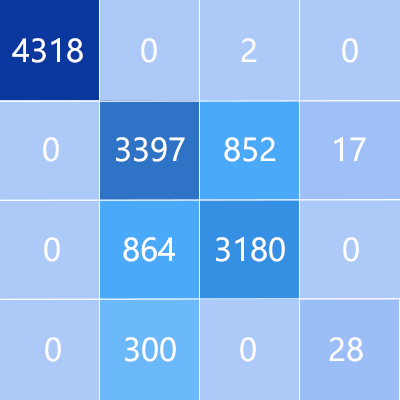
\includegraphics[width=.43\textwidth]{matrizconfusaosvm.png}&
            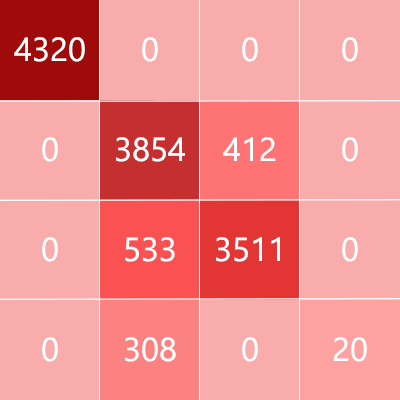
\includegraphics[width=.43\textwidth]{matrizconfusaobayes.png}
        \end{tabular}
        \caption{A esquerda encontra-se a matriz de confusão para a base de dados \textit{Nursery} utilizando do classificador SVM. A direita, a matriz de confusão para a mesma base, porém, utilizando do classificador \textit{Naïve Bayes}. Para as duas matrizes, as linhas e colunas estão representadas como segue: \textit{not\_recom}, \textit{priority}, \textit{spec\_prior}, \textit{very\_recom}.}
        \label{fig:matconfusao}
    \end{figure}

    Por fim, analisando os dois classificadores, podemos afirmar que o \textit{Naïve Bayes} foi superior na tarefa de classificação para as três bases de dados apresentadas nesse trabalho. Este obteve um melhor desempenho na maioria das métricas de análise de classificação abordadas.  Além disso, em média, este classificador foi 4\% melhor em comparação com o classificador SVM onde a maior diferença foi de 6,04\% para a base de dados \textit{Nursery} e a menor foi de 1,35\% para a base \textit{Mushrooms}.
    
    Os problemas aqui abordados, possuem números relativamente baixos de classes e atributos por amostra. Estes fatores influenciam diretamente na execução dos algoritmos visto que o algoritmo do \textit{Naïve Bayes} é preferível em situações as quais apresentam problemas pequenos. Dessa forma, o comportamento aqui encontrado de ambos algoritmos pode ser declarado como esperado, onde para os problemas apresentados o algoritmo SVM obteve um bom desempenho, porém, não superando ao do algoritmo \textit{Naïve Bayes}.

\section{Conclusão} \label{conclu}
    Este trabalho visou realizar uma análise comparativa entre uma versão aqui implementada do algoritmo de classificação \textit{Naïve Bayes} e uma versão presente na literatura do algoritmo \textit{Support Vector Machies} (SVM). Para isso, três bases de dados foram utilizadas: \textit{Car Evaluation Database}, \textit{Mushroom Database} e \textit{Nursery Database}. Estas, foram divididas em 10 \textit{folds} seguindo a técnica do \textit{k-folds cross-validation} e classificadas. Com as predições calculadas, as matrizes de confusão foram montadas e então, métricas de análise de classificadores foram aplicadas. Ao fim deste trabalho, pôde ser observado que para o contexto trabalhado e para os problemas abordadas, o algoritmo de classificação \textit{Naïve Bayes} obteve um melhor desempenho. Das métricas de análise utilizadas, este obteve valores superiores ao SVM. Quando observadas as acurácias encontradas, a implementação aqui desenvolvida de \textit{Naïve Bayes} apresentou em média 4\% de acertos a mais que o algoritmo do SVM. Onde no maior caso a diferença encontrada foi de 6,04\% utilizando-se da base de dados \textit{Nursery} e a menor diferença foi de 1,35\% para a base \textit{Mushrooms}. Destaca-se que o melhor valor de acurácia encontrado, foi alcançado utilizando-se de \textit{Naïve Bayes} com a base de dados \textit{Mushrooms}. Aqui, a acurácia encontrada foi de 100\%. Este valor pode ser justificado pela disposição da base, onde a mesma possui apenas duas classes, as quais possuem diferenças discrepantes em suas amostras e estas possuem um baixo nível de variabilidade.

\bibliographystyle{sbc}
\bibliography{sbc-template}

\end{document}
